\section{Resultados e Discussões}
Através da pesquisa realizada foi obtido informações referentes dos usuários sobre o uso das ferramentas de gerenciamentos de projetos conforme descrito a seguir:

Uma parte das empresas que trabalham com projetos colaborativos, uma parcela significativa não utilizam uma ferramenta de gestão, como evidenciado na Figura \ref{fig:useOnJob}, onde o gráfico com as respostas de pessoas entrevistadas na pesquisa, indicando que não utilizam qualquer tipo de ferramenta para esse fim.

\begin{figure}[H]
	\centering
	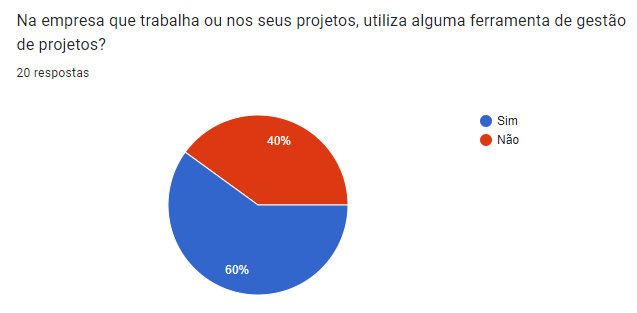
\includegraphics[width=300pt]{img/fig2.png}
	\caption{Utilizam ferramentas no ambiente de trabalho.}
	\label{fig:useOnJob}
\end{figure}

A falta de conhecimento por parte dos entrevistados, sobre conhecimento das metodologias ágeis, conforme ilustrado na Figura \ref{fig:scrumKnowledge}.

\begin{figure}[H]
	\centering
	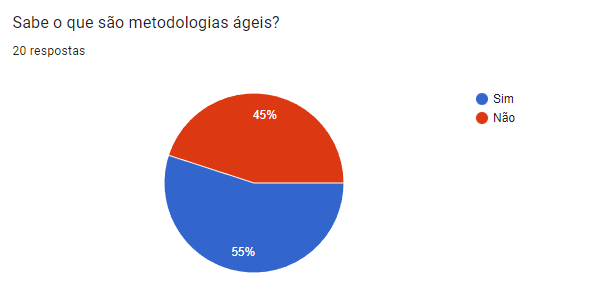
\includegraphics[width=300pt]{img/fig3.png}
	\caption{Conhecimento de metodologias ágeis.}
	\label{fig:scrumKnowledge}
\end{figure}

A figura \ref{fig:erModel} retrata a modelagem utilizada para a construção do banco de dados da aplicação

\begin{figure}[H]
	\centering
	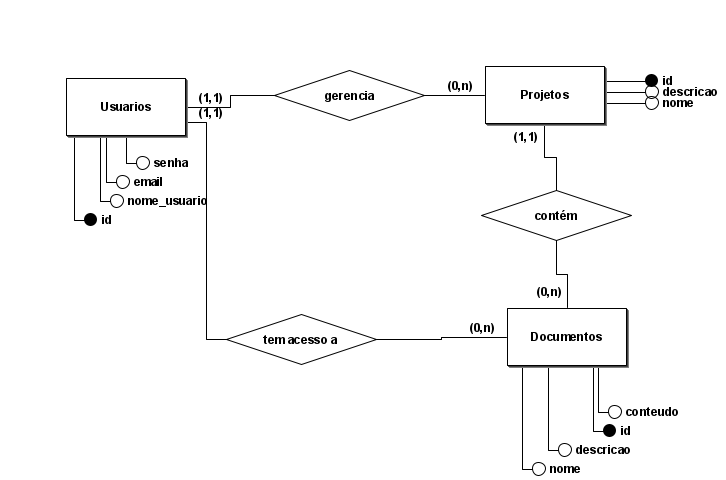
\includegraphics[width=300pt]{img/er-model.png}
	\caption{Modelagem do banco de dados}
	\label{fig:erModel}
\end{figure}

% No protótipo foi desenvolvida a funcionalidade de login do usuário, permitindo o acesso a uma tela principal onde será possível criar novos projetos, documentos e compartilhá-los com outros usuários. A Figura \ref{fig:login} ilustra essa tela de login.

% \begin{figure}[H]
% 	\centering
% 	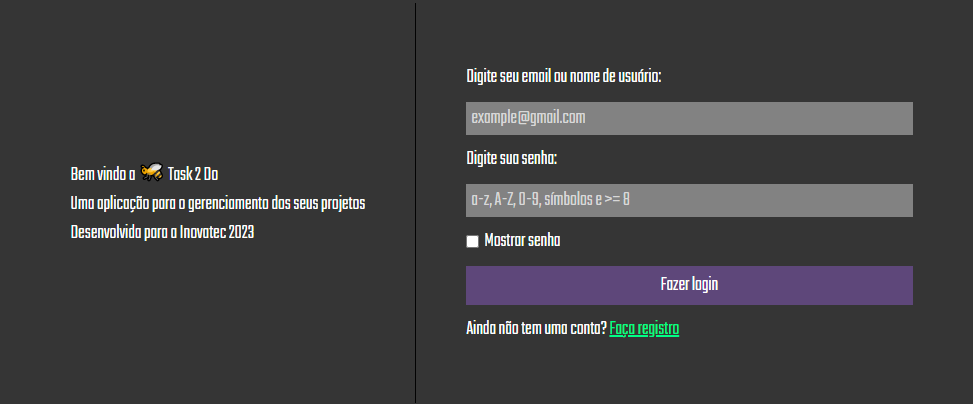
\includegraphics[width=350pt]{img/login.png}
% 	\caption{Tela de login}
% 	\label{fig:login}
% \end{figure}

A tela principal conta com o detalhamento dos projetos do usuário, conforme detalhada na Figura \ref{fig:app}, mostra todos os projetos criados pelo usuário e os documentos compartilhados com o mesmo, oriundos de outros projetos

\begin{figure}[H]
	\centering
	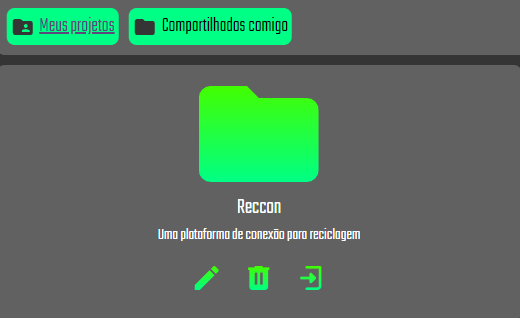
\includegraphics[width=350pt]{img/app.png}
	\caption{Componente de projetos}
	\label{fig:app}
\end{figure}

% Nesta seção do software, é possível visualizar todos os projetos pertencentes a um usuário, assim como os documentos compartilhados com outros colaboradores. Isso demonstra a eficiência da ferramenta no contexto do trabalho colaborativo, facilitando o acesso e o compartilhamento de informações entre os membros da equipe, conforme Figura \ref{fig:share}.

% \begin{figure}[H]
% 	\centering
% 	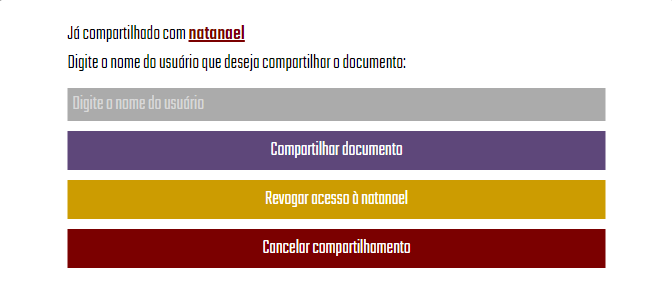
\includegraphics[width=350pt]{img/share.png}
% 	\caption{Tela de compartilhamento de documentos}
% 	\label{fig:share}
% \end{figure}

Ao final do processo tivemos vários cenários de testes que foram realizados para validar a integração dos projetos com os usuários e a verificação de possíveis inconsistências para que as correções necessárias fossem ajustadas de forma que o software realizasse os processos de forma ágil e colaborativa.

